\documentclass{article}
\usepackage[margin=1in]{geometry}
\usepackage{microtype}
\usepackage{setspace}
\usepackage{amsmath}
\usepackage{parskip}
\usepackage{amssymb}
\usepackage{graphicx}

\graphicspath{{../public/}}

\parskip=4ex
\date{}
\author{}

\title{12.6 Triple Integrals in Cylindrical Coordinates}

\begin{document}
  \maketitle
  \textbf{Introduction}\\
  In three dimensional dimensions, there is a coordinate system known as cylindrical coordinates, similar to polar coordinates. Some triple integrals are much easier to evaluate in cylindrical coordinates.

  \textbf{Cylindrical Coordinates}\\
  In cylindrical coordiante systems, a point $ P $ in three-dimensional space is represented by the ordered triple $ (r,\theta, z) $, where $ r ~\&~ \theta $ are polar coordinates of the projection $ P $ onto the $ xy $ plane and $ z $ is the directed distance from the $ xy $ plane to $ P $.

  Below is a diagram showing the cylindrical coordinates of a point $ P $ 

  \begin{center}
    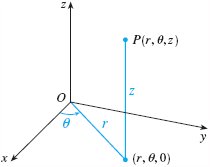
\includegraphics[width=6cm]{12_6_1}
  \end{center}

  To convert from cylindrical to rectangular coordinates, we use the equations
  \[
    x=r\cos{\theta} \qquad y=r\sin{\theta} \qquad z=z
  \]
  
  While to convert from rectangular to cylindrical coordinates, we use
  \[
    r^{2}=x^{2}+y^{2} \qquad \tan{\theta}=\frac{y}{x} \qquad z=z
  \]

  \textbf{Ex 1}\\
  A) Convert the cylindrical coordinates $ (2,\frac{2\pi}{3},1) $ to rectangular coordinates
  \[
    \begin{gathered}
    x=2\cos{\frac{2\pi}{3}}=-1\\
    y=2\sin{\frac{2\pi}{3}}=\sqrt{3}\\
    z=1\\
    ~\\
    \boxed{(2,\frac{2\pi}{3}) \to (-1,3,1)} 
    \end{gathered}
  \]

  B) Find cylindrical coordinates of the point with rectangular coordinates $ (3,-3,-7) $
  \[
    \begin{gathered}
    r=\sqrt{3^{2}+(-3)^{2}}=3\sqrt{2}\\
    \tan{\theta}=\frac{-3}{3}=-1 \qquad \theta=\frac{7\pi}{4}+2n\pi\\
    z=-7\\
    \boxed{(3,-3,-7) \to (3\sqrt{2},\frac{7\pi}{4}+2n\pi,-7)}
    \end{gathered}
  \]

  Because of $ \theta $ not being a constant and rather a function, there are multiple sets or triples of cylindrical coordinates.

  \textbf{Evaluating Triple Integrals with Cylindrical Coordinates}
  \[
    \INT*{^{},_E,^{}}f(x,y,z)~dV = \int^{\beta}_{\alpha} \int^{h_2(\theta)}_{h_1(\theta)} \int^{u_2(r\cos{\theta},r\sin{\theta})}_{u_1(r\cos{\theta},r\sin{\theta}} f(r\cos{\theta},r\sin{\theta},z)r ~dzdr\theta 
  \]

  I is optimal to use this formula when $ E $ is a solid region easily described in cylindrical coordinates and especially when the function $ f(x,y,z) $ involves the expression $ x^{2}+y^{2} $ 
  
  \textbf{Ex 2}\\
  A solid $ E $ lies within the cylinder $ x^{2}+y^{2}=1 $, below the plane $ z=4 $, and above the paraboloid $ z=1-x^{2}-y^{2} $. The density at any point is proportional to its distance from the axis of the cylinder. Find the mass of $ E $

  In cylindrical coordinates,
  \[
    E=\{ (r,\theta,z) | 0 \le \theta \le 2\pi, 0 \le r \le 1, 1-r^{2} \le z \le 4\}
  \]

  Since density at $ (x,y,z) $ is proportional to the distance from the $ z $ axis, the density function is
  \[
    f(x,y,z)=K\sqrt{x^{2}+y^{2}}=Kr 
  \]

  where $ K $ is the proportionality constant
  \[
    \begin{gathered}
      m=\INT*{^{},_E,^{}}K\sqrt{x^{2}+y^{2}}~dV= \int^{2\pi}_{0} \int^{1}_{0} \int^{4}_{1-r^{2}} (Kr) r~ dzdrd\theta = \boxed{\frac{12\pi K}{5}} 
    \end{gathered}
  \]
  
   \textbf{Ex 3}\\
   Evaluate $ \int^{2}_{-2} \int^{\sqrt{4-x^{2}}}_{-\sqrt{4-x^{2}}} \int^{2}_{\sqrt{x^{2}+y^{2}}} x^{2}+y^{2} ~ dzdydx $ 
  \[
    \begin{gathered}
    E=\{ (x,y,z) | -2 \le x \le 2, -\sqrt{4-x^{2}} \le y \le \sqrt{4-x^{2}}, \sqrt{x^{2}+y^{2}} \le z \le 2 \}\\
    \to\\
    E=\{ (r,\theta,z) | 0 \le x \le 2\pi, 0 \le y \le 2, r \le z \le 2 \}\\
    ~\\
    \INT*{^{},_E,^{}} x^{2}+y^{2}~dV\\
    \int^{2\pi}_{0} \int^{2}_{0} \int^{2}_{r} r^{2}r ~ dzdrd\theta\\
    \int^{2\pi}_{0} d\theta \int^{2}_{0} 2r^{3}-r^{4} ~ dr\\
    2\pi \text{\huge{[}} \frac{1}{2}r^{4}-\frac{1}{5}r^{5} \text{\huge{]}}^{2}_0=\boxed{\frac{16}{5}\pi}
    \end{gathered}
  \]
\end{document}
